\section{Le développement}
\subsection{Gestion de l’inventaire matériel}
La gestion de l'inventaire est l'un des aspects essentiels de la GMAO. 
Elle consiste à suivre et à contrôler les matériel afin de maintenir les 
actifs en bon état de fonctionnement. Les responsables et les techniciens de la maintenance peuvent ,
à l'aide d'un formulair dédié, de faire rentrer dans le système les nouveau matériels.

Pour cela, un module a été créé pour que 
les administrateurs puisse ajouter, modifier ou supprimer des matériels. 
Ce module est constitué d’un formulaire dans lequel l’administrateur 
saisira les informations nécessaires à la création d’un matériel. 
Ces informations sont le numéro de série, la famille d’appartenance, le nom, 
le modèle de matériel auquel il est rattaché, le fournisseur, une description, la localisations
dans laquelle ce matériel se situe au sein des déffirents site de laboratoir et 
les dates d'expiration (si pertinent)
\begin{figure}[hp]
    \centering
    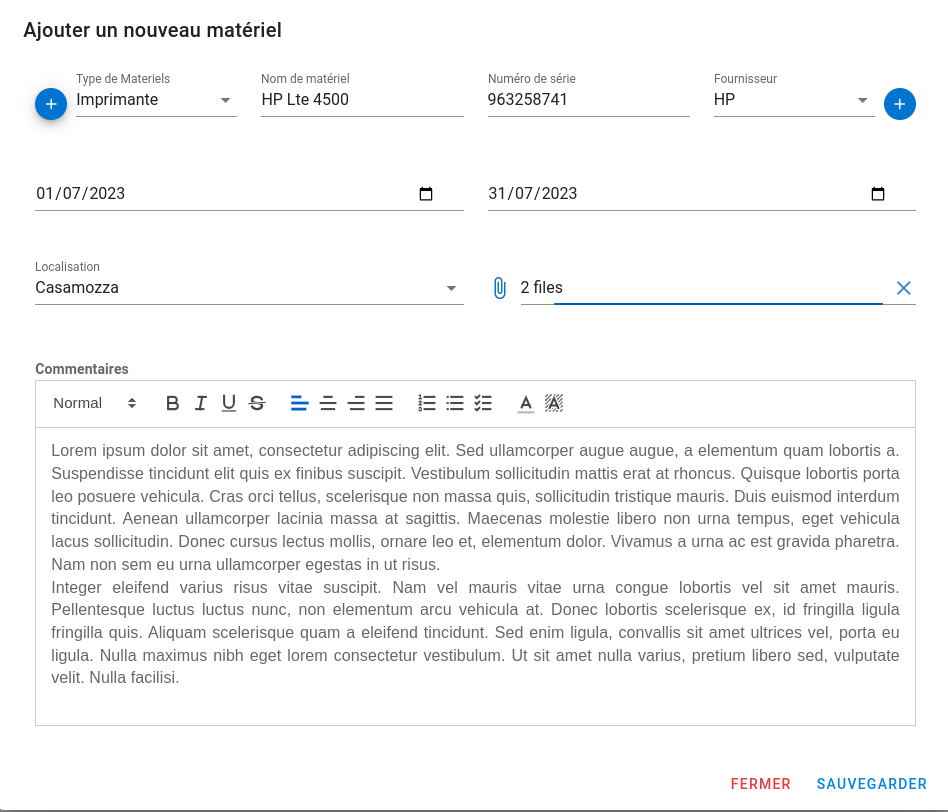
\includegraphics[width=400pt, height=400pt]{images/inventaire.png}
    \caption{Formulaire de saisie de matériel}
\end{figure}

\subsection{Planification des activités de maintenance}
La planification des activités de maintenance dans une GMAO est un processus complexe 
qui nécessite une attention méticuleuse aux détails et une collaboration étroite 
entre les différents acteurs impliqués dans la gestion de la maintenance. 
Une bonne planification permettra d'assurer la disponibilité et la fiabilité 
des équipements, ce qui contribuera à améliorer l'efficacité opérationnelle et 
à réduire les coûts de maintenance.
\subsubsection{Les opérations:}
Une opération est un document électronique 
qui décrit les détails d'une tâche ou d'une activité de maintenance à effectuer. 
Il s'agit d'une instruction formelle donnée à une équipe de maintenance ou 
à un technicien pour exécuter des travaux spécifiques sur un équipement, 
une machine ou un système.

les éléments généralement inclus dans une opération d'une GMAO :
\begin{itemize}
    \item Identifiant : Un numéro ou une intitulé unique attribué àl'opération pour 
    le suivi et la référence.
    \item Description de la tâche : Une explication détaillée des travaux à effectuer, 
    y compris les étapes spécifiques et les instructions nécessaires pour accomplir la 
    tâche.
    \item Équipement concerné : Le nom, le numéro de série et/ou l'identification de 
    l'équipement ou de la machine nécessitant la maintenance.
    \item Commentaires et remarques : Des notes supplémentaires sur l'état d'avancement 
    des travaux ou d'autres informations pertinentes.
\end{itemize}
\begin{figure}[hp]
    \centering
    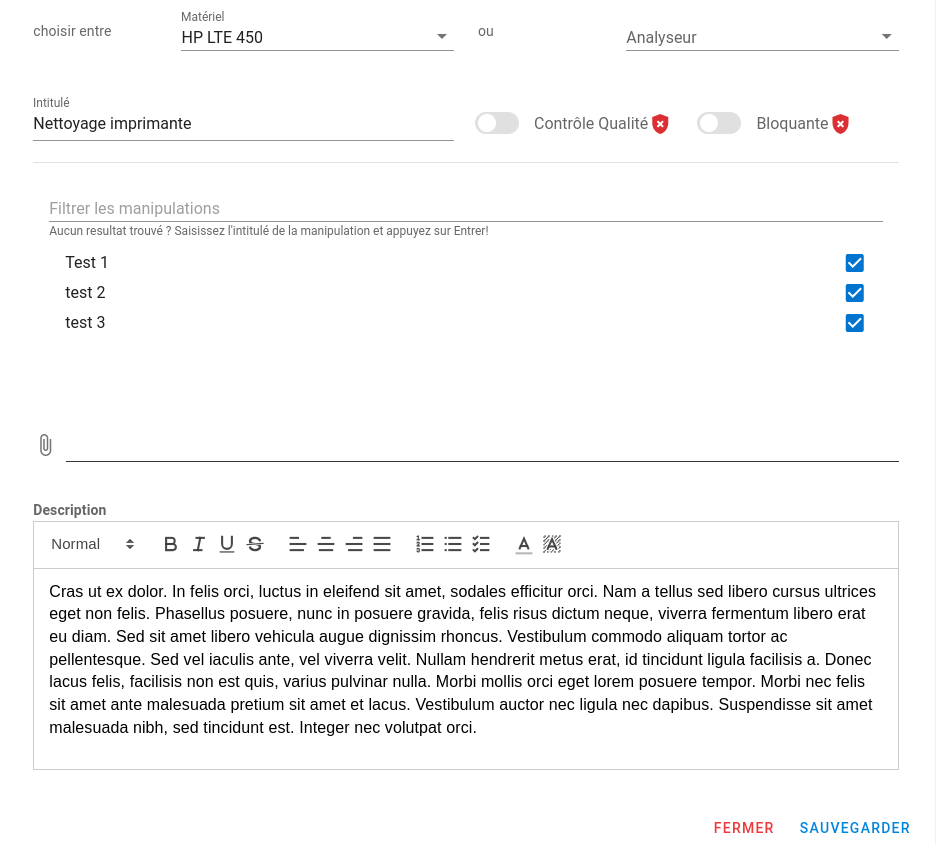
\includegraphics[width=300pt, height=220pt]{images/operation_settings.png}
    \caption{Formulaire de saisie d'opérations}
\end{figure}

Ces opérations permettent de suivre et de gérer efficacement les activités de maintenance, d'assurer 
la communication entre les membres de l'équipe et de garantir que les travaux sont 
effectués de manière cohérente et méthodique.
\subsubsection{Les interventions}
Les interventions dans une GMAO permettent d'assurer la maintenance préventive et 
curative des équipements, d'améliorer leur disponibilité et leur efficacité, tout en 
réduisant les temps d'arrêt non planifiés et en augmentant la durée de vie des actifs 
de l'entreprise.

Les interventions font référence aux différentes actions de maintenance réalisées sur 
les équipements, machines ou installations d'une entreprise. Ces interventions sont 
enregistrées, suivies et gérées par le système GMAO pour assurer un suivi efficace de 
la maintenance.

Les étapes typiques d'une intervention dans une GMAO :
\begin{itemize}
    \item Création de la demande d'intervention : Lorsqu'un problème est détecté sur un équipement ou lorsqu'une maintenance préventive doit être effectuée, une demande d'intervention est créée dans la GMAO. Elle peut être générée automatiquement par le système en fonction des plannings de maintenance ou saisie manuellement par un opérateur.
    \item Assignation de l'intervention : La demande d'intervention est attribuée à un technicien ou une équipe de maintenance appropriée. L'affectation peut être basée sur les compétences requises, la disponibilité du personnel et la localisation géographique.
    \item Planification : Une fois l'intervention attribuée, elle est planifiée dans le calendrier de maintenance. La date et l'heure de l'intervention sont définies en tenant compte des priorités, de l'urgence et de la disponibilité des ressources.
    \item Exécution de l'intervention : Le technicien ou l'équipe se rend sur le site de l'intervention et effectue les tâches de maintenance requises. Cela peut inclure des réparations, des remplacements de pièces, des vérifications, des réglages, etc.
    \item Saisie des données : Pendant l'exécution de l'intervention, le technicien enregistre les informations pertinentes dans la GMAO. Cela peut inclure les heures de travail, les pièces utilisées, les observations sur l'état de l'équipement, les actions effectuées, etc.
    \item Validation : Une fois l'intervention terminée, le travail est vérifié et validé par un responsable ou une équipe de contrôle de qualité pour s'assurer que toutes les tâches ont été correctement exécutées.
\end{itemize}
\pagebreak
\subsection{Le calandrier des interventions}
Les techniciens ou les èquipes de la maintenance peuvent visualizer, selon leurs droits d'utilisateur
ou leur affectations, un calandrier regroupant les tâches à effectuer dans dans la journée, la semaine, le mois etc.

Ce calandrier permets la suivie de l'avancements de toutes les tâches de la maintenance en cours,
ainsi que une vision globale sur toute les retards potentiels ou les changements de dates heurs etc..
\begin{figure}[hp]
    \centering
    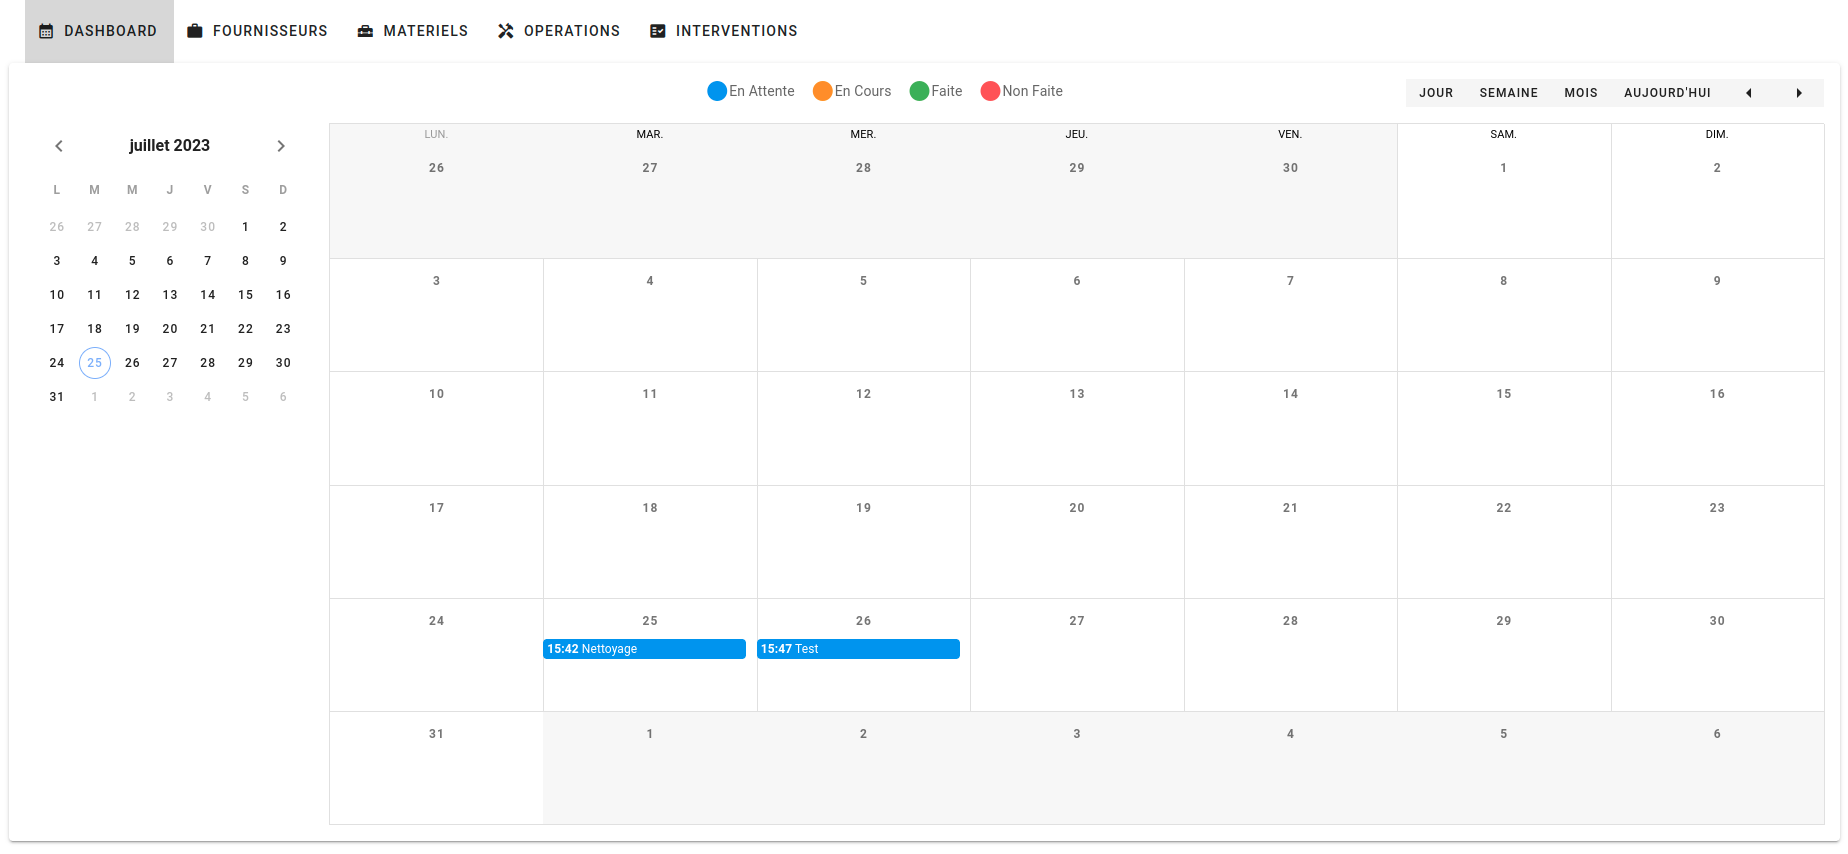
\includegraphics[width=450pt, height=400pt]{images/dashboard.png}
    \caption{Le calandrier des interventions}
\end{figure}
\pagebreak